\documentclass{article}
\usepackage{geometry}   
\geometry{letterpaper, margin=1in}
\usepackage[english]{babel}
\usepackage[utf8x]{inputenc}
\usepackage{bbm}
\usepackage{amsmath}
\usepackage{amsfonts}
\usepackage{units}
\usepackage{mathrsfs}
\usepackage{tikz}
\usepackage{bm}
\usepackage{dsfont}
\usepackage{setspace}
\usepackage{makecell}
\graphicspath{ {./images/} }

\title{Price Theory 1 - Problem Set 2 - Question 2}
\author{Timothy Schwieg \and Samuel Barker \and Rafeh Qureshi \and Ana Vasilj
 \and Daniel Noriega}

\begin{document}

\maketitle

\section{Question: Cigarette tax/ban with an outside market}

This is a partial equilibrium setting where we are looking only at the
cigarette market: the legal and the illegal one which are linked via
the market price for cigarettes. There are five types of homogeneous
agents: adult smokers, adolescent smokers (demand side), legal and
illegal cigarette producers (supply side) and the government who
collects the tax revenue We know that:

\underline{Production side:}
\begin{itemize}
\item legal cigarettes produced and distributed at a constant marginal
  cost c
\item (assume) there is a unit per-cigarette tax $\tau$ levied on the
  production side [due to the tax equivalence result we know it does
  not matter which side of the market they are levied from]
\item only way to avoid the taxes is to produce and sell cigarettes
  illegally
\item illegal producers exist in the marketplace, but have a small
  market share
\end{itemize}

\underline{Consumption side:}
\begin{itemize}
\item elasticity of demand of cigarettes with respect to its retail
  price is around -1/2
\item cigarettes are harmful to a smoker's health - assume a cost to
  an individual = k per cigarette (in monetary terms)
\item we will assume that cigarettes are also harmful for other
  individuals and impose a constant negative health externality on
  society equal to a constant h per cigarette (in monetary terms)
\end{itemize}



\subsection{How is it possible for tax-free illicit cigarettes to
  coexist with taxable cigarettes? What are some of the variables
  determining the market shares of those two products?}

It is reasonable to assume that there are \textit{fixed repercussions
  for being caught selling illegal cigarettes} (assume buyers are
always unpunished because the legal and illegal cigarettes are
indistinguishable). We can also assume that the \textit{probability of
  being caught rises exponentially with the amount of
  cigarettes that the criminals are selling} (i.e. with the absolute
size of the illegal market). Note, that we could also have the case where the illegal market is
also perfectly elastic, due to free entry and a fixed cost on users through the punitive measures; we believe
the case of the governments raising their punishments and search efforts with increases in the quantity of illegal 
drugs supplied a more reasonable one.
If criminals are risk neutral and
perceive the additional costs as \underline{Pr(getting
  caught)$\times$repercussions}, their marginal cost of producing each
additional cigarette will be rising linearly with the amount of
cigarettes produced. Assume that the underlying ``production
technology" is the same in the illegal market so that- without taking
into account the probability of getting caught and the punishment -
both producers have the same marginal cost c.

Assuming perfect competition in the legal market means that profits
are zero and the legal supply is perfectly elastic at price p* = c +
$\tau$. Conversely, due to the rising marginal cost of producing and
selling each additional cigarette in the illegal market, criminal
supply will be upwards sloping (starting from the constant cost c) and
will cross the legal supply curve at (p*=c+$\tau$, $x_{illegal}$).

Assuming that individuals are indifferent between legal and illegal
cigarettes (identical) that are sold at the same price, criminals
cannot charge a price higher than the legal p*=c+$\tau$, otherwise
everyone would just buy the cheaper legal cigarettes. It would also be
suboptimal for the criminals to sell them for less. Thus, criminals
will be selling $x_{illegal}$ cigarettes at the price
$p^{*}=p_{illegal}=c+\tau$.

\centerline{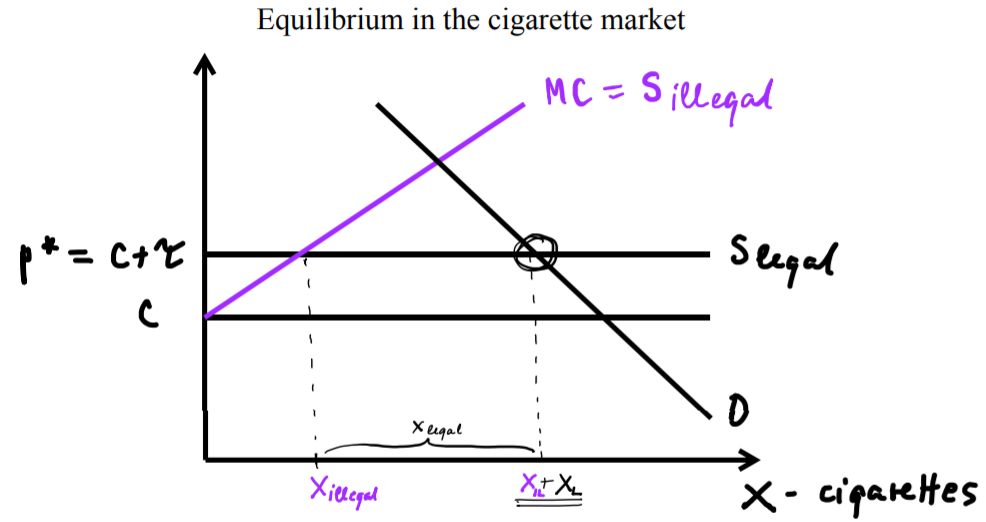
\includegraphics[width=.5\textwidth]{graph1.png}}

In this set-up, the market share of illegal cigarettes will depend on:
\begin{itemize}
\item how steep the illegal supply curve is - i.e. how much does the
  risk of getting caught increase with each additional cigarette
  illegally sold (market share decreases with $\partial MC_{illegal}/\partial$x)
\item size of the tax ($\tau$) relative to the marginal cost of
  production $c$, which reflects the size of the "comparative
  advantage" of the illegal production of cigarettes that is un-taxed
  (market share increases with $\tau$)
\end{itemize}

We could also imagine that, maybe, consumers prefer to buy legal
cigarettes and will have to be compensated by a lower price
$p_{illegal}$ = p*-$\delta$ to buy illegal ones. In this case, the illegal
market share would be inversely proportional to $\delta$. Nevertheless, we
omit that from further analysis because the parameter itself does not
add any new insights. 

\subsection{TRUE/FALSE/UNCERTAIN. The small size of the illicit market
  is good evidence that a ban on cigarettes would eliminate the
  majority of smoking.}

This statement is uncertain - it depends on what the tax $\tau$ relative
to the marginal cost $c$ is, or where the intersection of the demand
function with the constant marginal cost $c$ is, among others.

We know from the set-up of the question that the illegal market share
is small. This could be due to a low tax $\tau$ (low "comparative
advantage" of illegal sales) or due to a high slope of the supply (MC)
curve for the illegal producers (risks of getting caught increase
quickly with the amount sold).

If we know that the taxes are sufficiently high relative to the
marginal cost $c$- and there is a a low market share - this means that
banning cigarettes will reduce the majority of smoking because we can
infer that the illegal supply curve is very steep. $->$ We could infer
that the statement would be TRUE

If we know that the taxes are low - and there is a a low market share
- it might be the case that the supply curve of criminals is fairly
flat (low risk of getting caught as production increases) $->$ In
which case the statement will most likely be FALSE

% (GRAPH - 2 graphs - show 2 cases)
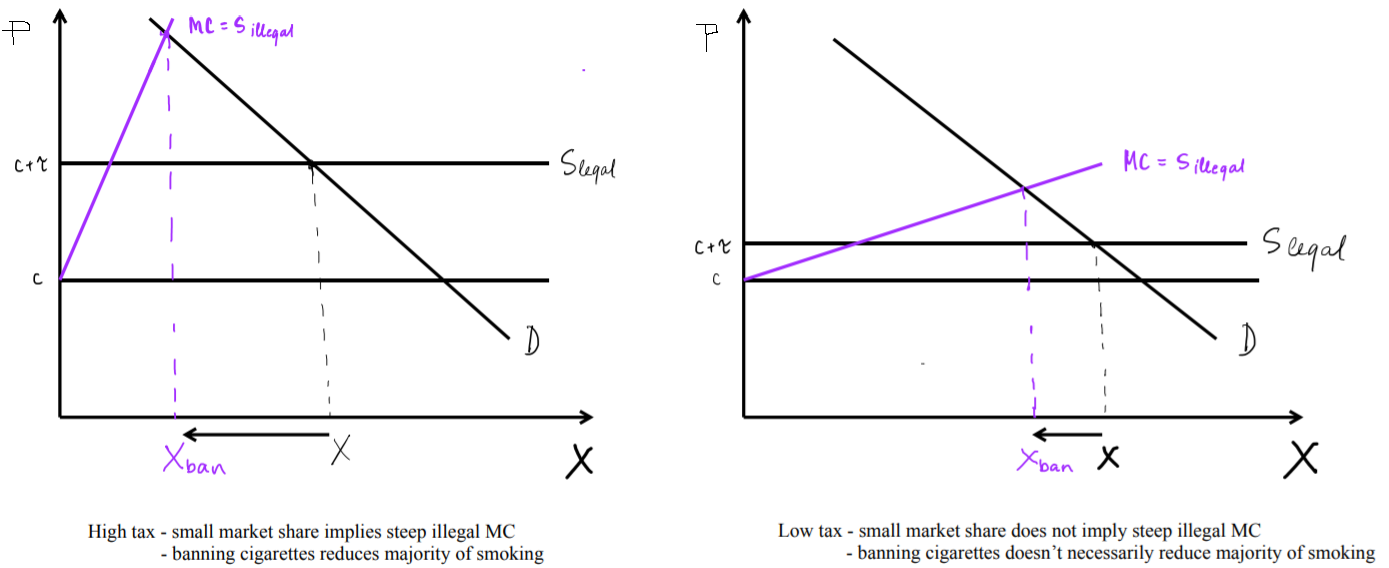
\includegraphics[width=.9\textwidth]{Graph2.png}


\subsection{Suppose the health cost of each cigarette exceeds the
  amount of the excise tax.}
\subsubsection{Is it socially beneficial to ban cigarettes? Does it
  matter whether ``social benefit" includes the welfare of criminals?}

What should we assume the tax $\tau$ to be? Obviously, from the question,
it could be anything which is lower than the overall health cost of
one cigarette on both the smoker(k) and the environment(h). Still,
unless the government has some irremovable revenue requirement which
might induce it to impose inefficient taxes, a very reasonable
assumption would be that the government set them to be equal to the
marginal externality of cigarette smoke imposed on society per
cigarette (h) - which would be the optimal (Pigouvian) tax in a
legal-market-only world. Since:

$$\text{Total health cost per cigarette = cost to the smoker (k) + negative externality (h)}$$,

the optimal Pigouvian tax $\tau$=h is by default lower than the total
health cost of a cigarette h+k. So, let's assume - also for simplicity
of the forthcoming analysis - that the unit tax $\tau$ set by the
government is equal to the marginal externality of smoking h. Without
the illegal market, this would ensure that the smokers are faced with
the correct "social cost" of smoking a cigarette - and this would
eliminate the deadweight loss of the smoking externality h.

[Assume throughout that consumers have quasilinear preferences so that
we can measure deadweight losses/consumer surplus with the area under
the Marshallian demand curve]

With the illegal market, the tax $\tau$ = h still involves a deadweight
loss in the form of lost taxes (red triangle in GRAPH 1)

In this framework it is \textbf{definitely not socially beneficial to
  ban cigarettes}, no matter whether we include criminals'
welfare. \textbf{[This assumes that criminals are punished in a
  non-monetary way.]}

Whether we include criminal welfare or not will only affect how big
the total surplus drop is. \textbf{If we include criminals' welfare,
  it will make total welfare drop by less in the complete-ban case
  because they are the only ones whose welfare (producer surplus)
  increases with the complete ban}, because all the cigarettes are now
supplied by them and at a higher price than before.

The reduction in overall social welfare occurs because banning
cigarettes all-together means that \textbf{all cigarettes need to be
  obtained from the illegal sector, which is relatively inefficient in
  producing cigarettes because it involves the non-monetary punishment
  cost which induces a benefit to no one.} Conversely, the tax revenue
collected from legal producers goes into government revenue, which
could later be re-distributed to consumers and does not constitute
lost surplus.

Thus, \textbf{with the ban, there will be a production inefficiency,
  lost tax-revenue and a drop in consumer surplus (CS) - which cannot
  be overweighted by the increase in criminals' production surplus
  (PS). The increase in criminals' PS only partially offsets the drop
  in CS, while there are also lost taxes (red dots square) and
  "productively inefficient" violence (red/purple triangle)} (see
Graph and calculation below).
$$\text{Total surplus (TS) = Consumer Surplus +  Producer (criminal) Surplus + Tax Revenue - Health Cost}$$
$$TS1= A+B+E+C+D+E$$
$$TS2= A+B+E-G$$
Can see from the graphs why social welfare is always lower with a full
ban on cigarettes than with the Pigouvian unit tax $\tau$=h.


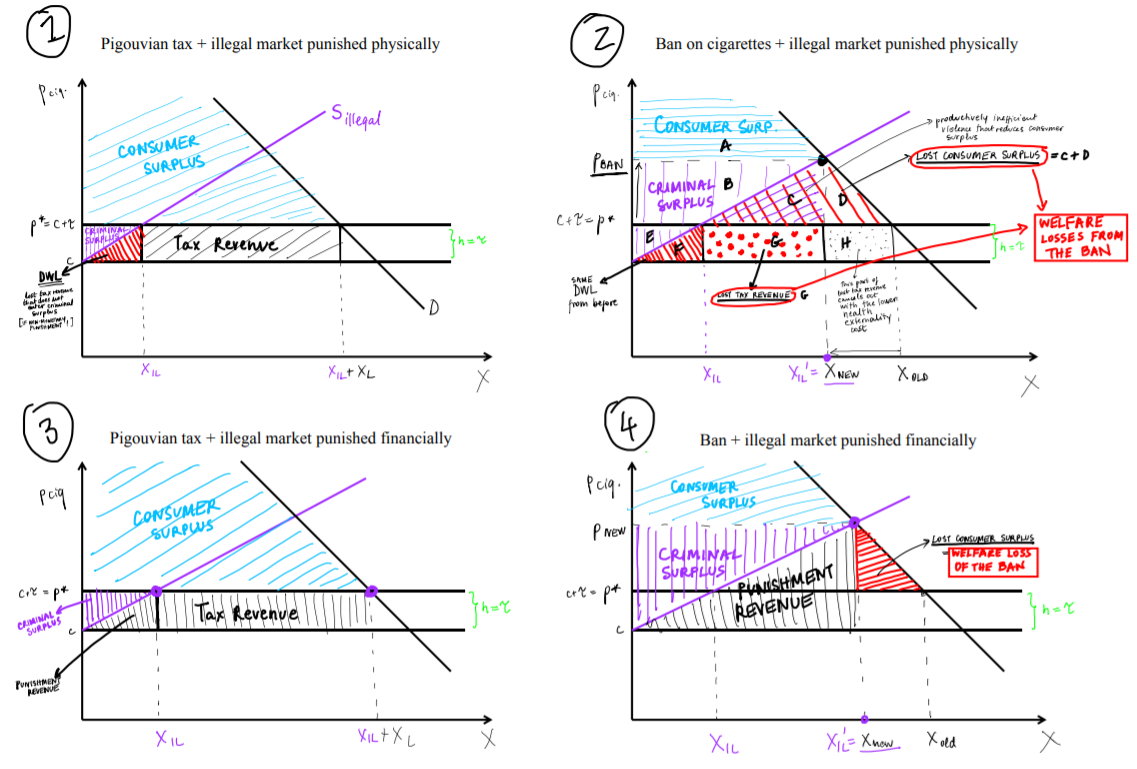
\includegraphics[width=\textwidth]{Graph3.png}

\subsubsection{Does it matter whether the criminals are punished
  monetary finer rather than prison, fines etc.?}

In short - yes and no.

\underline{Yes}, because punishing the criminals with violence is a
cost to the criminals but a benefit to no one. Conversely,
\textbf{punishing them with monetary fines} which would be (for the
criminals) equivalently as costly as violence/prison \textbf{increases
  the size of the pie}. The cost to the criminals stays the same,
while this cost is transferred directly as extra revenue (surplus) to
the government. So this is definitely better welfare-wise in both
cases (taxes or ban) than the violence/prison punishment.

\underline{No}, because it does not change the conclusion that
\textbf{taxes are still better than the ban}. Taxes accompanied with a
monetary punishment are actually Pareto optimal - no dead-weight losses
- while the ban imposes a dead-weight loss on the consumer-surplus side
(triangle B).

These results can be seen from the collection of graphs above.



\subsection{Retailers are currently prohibited from selling cigarettes
  to minors, and this prohibition is enforced with the same rules and
  resources that enforce excise-tax payment. What does economic theory
  say about \underline{whether} and \underline{how} minors receive
  their cigarettes?}

Let's look at demand from adults and minors separately. Assume that
adults do not buy the cigarettes for the minors, and that minors have
a similar demand function as adults.

This means that minors can acquire cigarettes only in the illegal
market. Therefore, illegal and legal cigarettes are not perfect
substitutes anymore--the condition that the price of legal and illegal
cigarettes has to be the same in equilibrium does not hold. Since
minors can only purchase cigarettes in the illegal market, they drive
up the price of illegal cigarettes by increasing their demand. Minors
crowd out adults buying illegal cigarettes because in order for minors
to acquire cigarettes kids must be willing to pay more than the legal
price.

As more minors buy illegal cigarettes, thereby increasing the illegal
price of cigarettes, more adults will buy cigarettes from the legal
market, which would also increase the tax revenue.

$$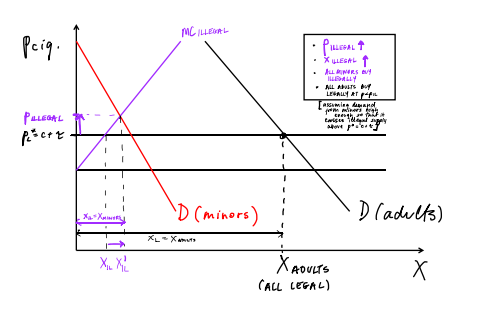
\includegraphics[width=.6\textwidth]{dudewheresmymodel.png}$$

\subsection{Would it be socially beneficial to legalize sales to
  minors?}

Assuming again that minors have a similar demand function as adults,
legalizing sales to minors would be equivalent to increasing the
demand side of the market base. There will be more
people willing to buy any quantity of cigarettes at a given price.

Since the marginal price of cigarettes $c$ is constant, the market
clearing price will be the same, but the quantity will increase by the
number of cigarettes that children are willing to purchase at that
price. Therefore, if no externalities were considered, society will be
strictly better off as consumer surplus would increase more than the
decrease in producer surplus (previous illegal surplus).

If externalities were considered, however, the specific effect on
total social surplus would be uncertain as it would depend on the
specific value and form (i.e. $functional form$) of the
externality. The main effects would be captured by the increase in
minor's consumer surplus, and the additional externality due to their
consumption.

$$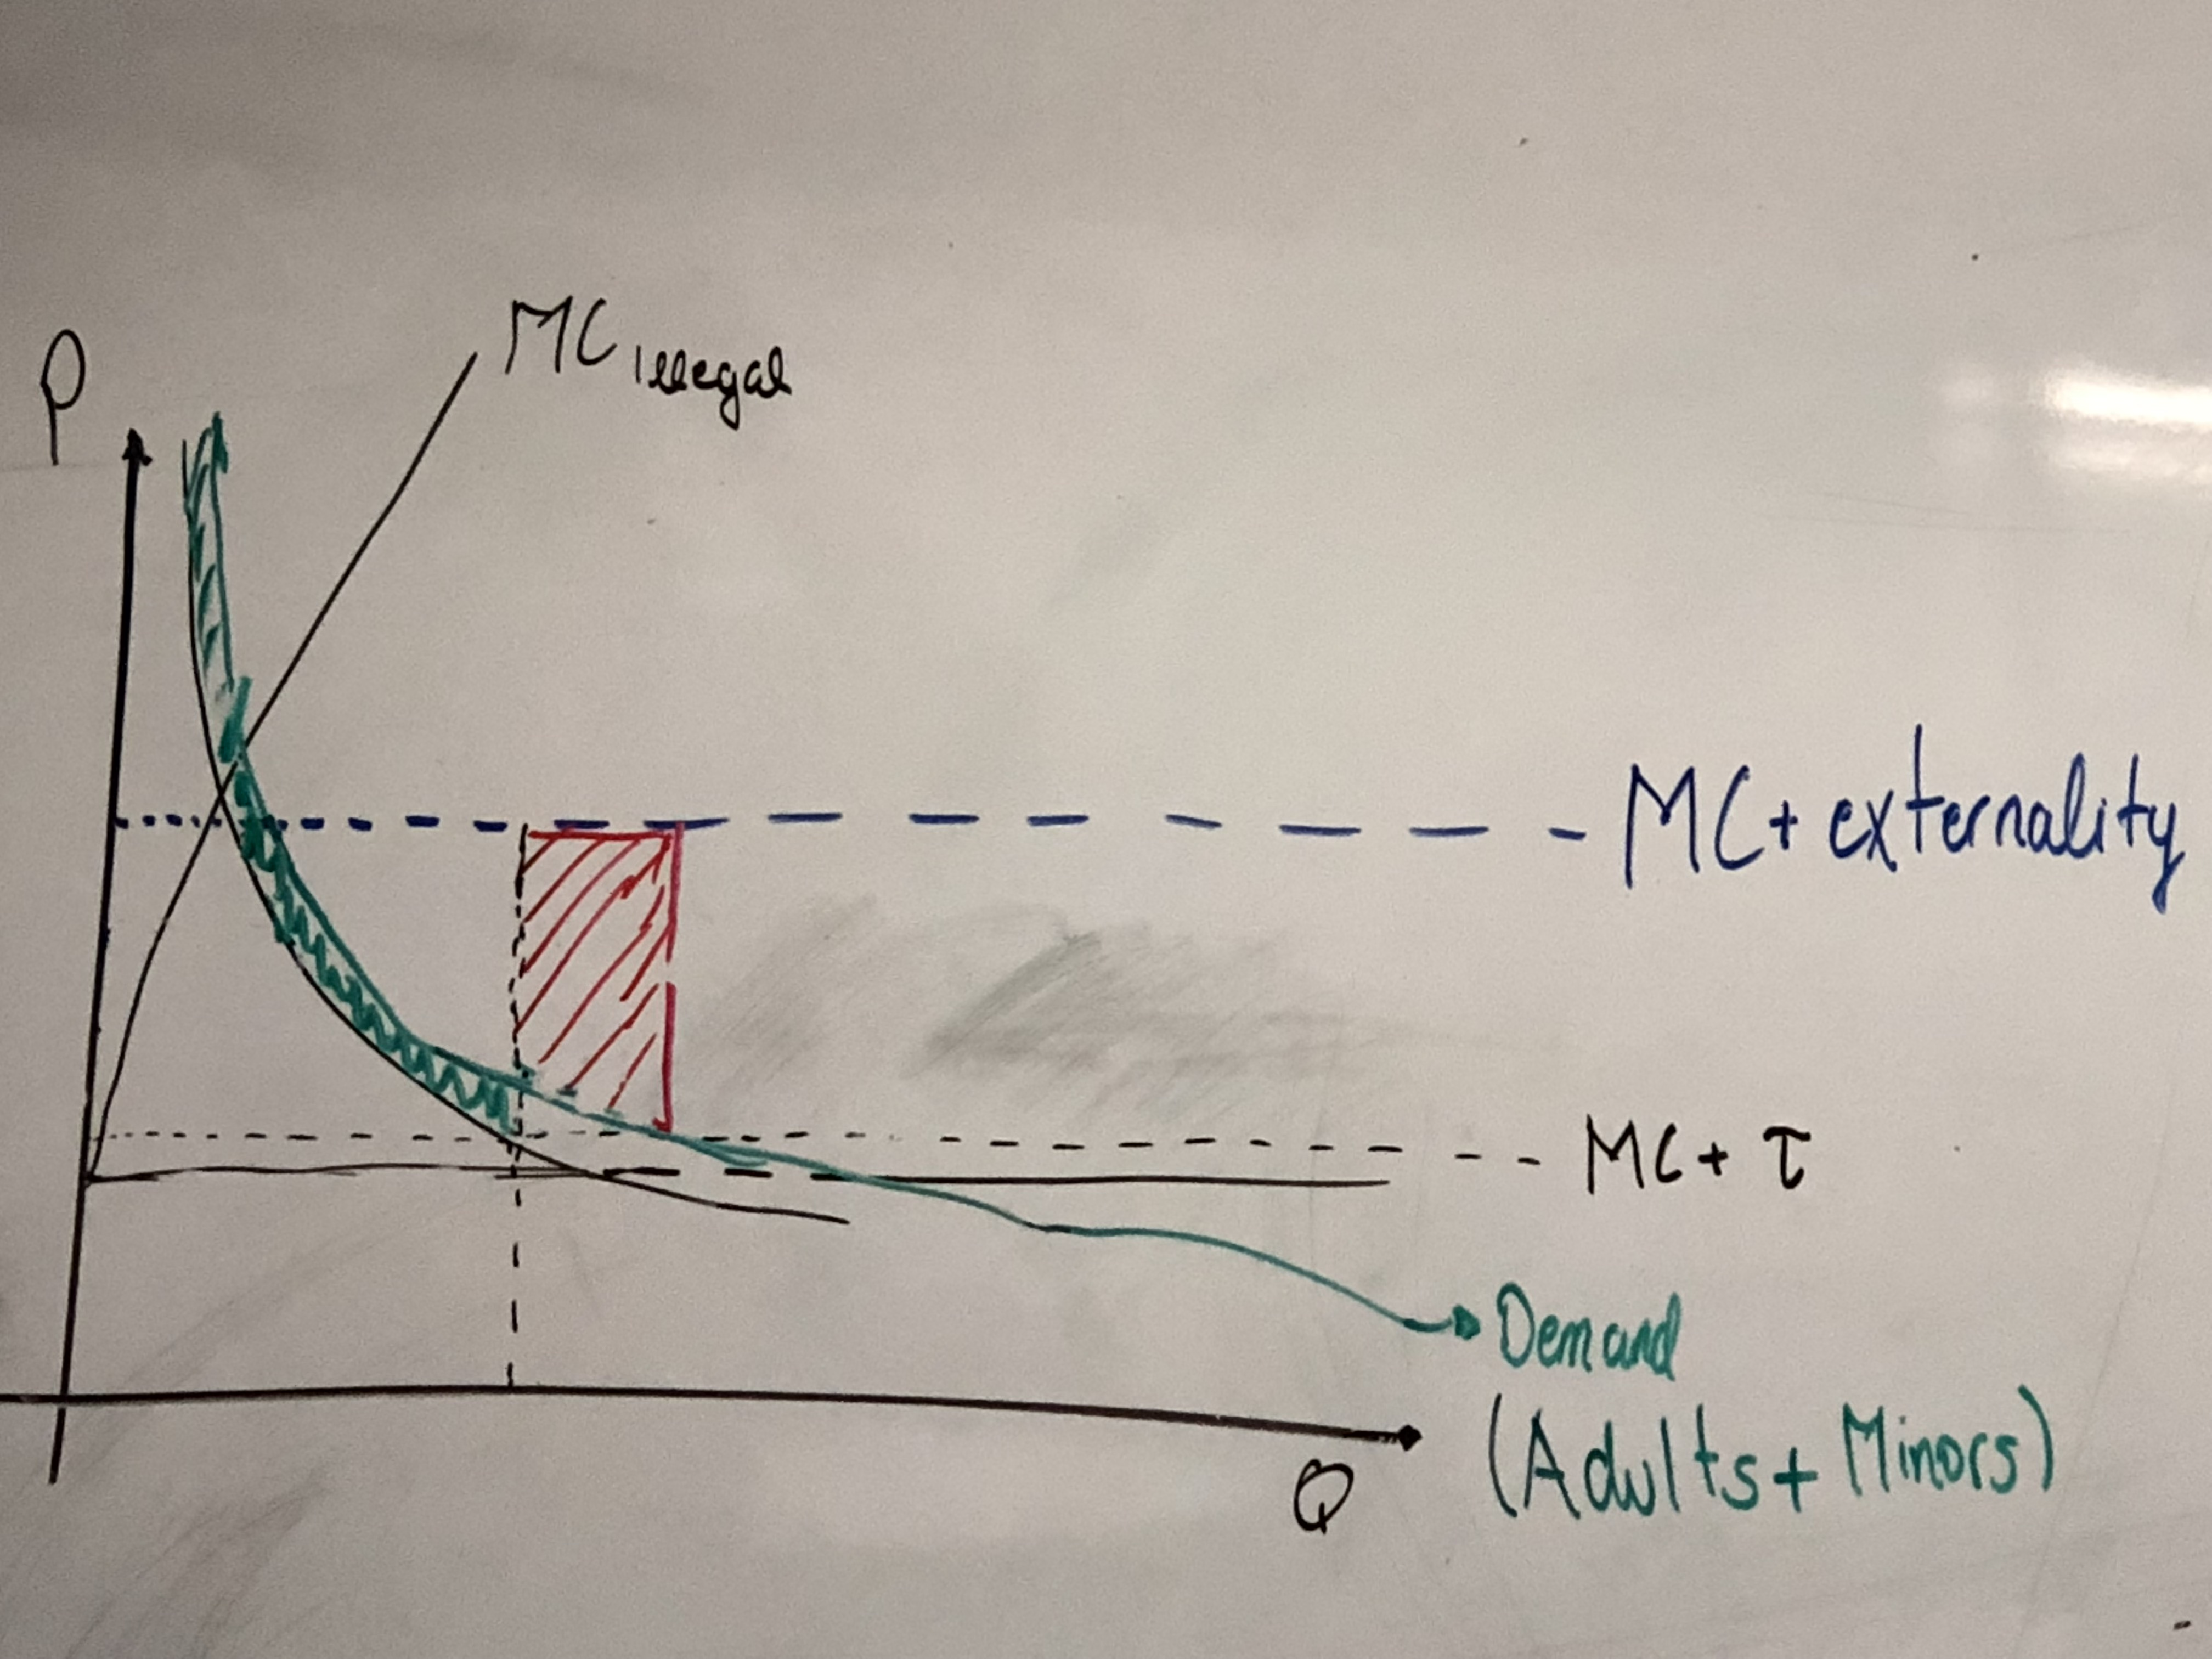
\includegraphics[width=.6\textwidth]{Daniel.jpg}$$

\subsection{If it were shown that minors were receiving their
  cigarettes from adults who were purchasing them from legitimate
  retailers, does that strengthen the case for prohibiting cigarettes
  for adults, too?}

Let's assume that the adults are completely willing to give
legally-purchased cigarettes to kids, and that this action entails zero cost
to the adults (no police knocking on their door if they give cigarettes
to minors).

This case is completely equivalent to legalizing cigarette sale to
minors. Illegal market sells at price p*=c+tax (Pigouvian tax equal
to smoking externality h). Quantity sold equal to
the amount adults+minors are willing to buy a the given market
price. No dead-weight  loss [IF we assume that minors smoking, per se,
does NOT represent a societal cost, and illegal sellers are punished
in a monetary way which ends up being government revenue] - the
cigarette market is Pareto efficient.

In this case it would, obviously, not be beneficial to impose a full
ban on cigarettes for everyone.

Still:

1) If there is some monetary risk (e.g. a fine which ends up as
government revenue) to adults for giving cigarettes to minors, and
minors have to pay a premium over the price p* to get the cigarettes,
then there will be a consumption inefficiency.Still, banning all
cigarettes would impose a worse inefficiency because everything would
be produced by the illegal sector (graph...)

2) If we believe kids smoking are imposing an externality to
themselves (too young/immature to understand the health cost, then
adults giving them cigarettes is also inefficient. If this externality
is very high and there are a lot of minors who demand cigarettes, then
there might be a trade-off question whether to ban cigarettes
all together or not.


\subsubsection{Would your answer be different if evidence showed that
  minors were stealing cigarettes from adults and from retailers?}

If minors are stealing cigarettes from RETAILERS, their marginal cost
of production, in expectation, goes up because of the stolen
cigarettes $$\text{Cost increase to legal producers =(no of cigarettes
  stolen*c}$$ This increase is directly transferred to minors. But there is a welfare
loss to adult consumers because now they have to pay a higher price
for each cigarette purchased in the legal market. There is also a
health externality equal to (no. of minor cigarettes*h) which is not
compensated by tax revenue because kids do not have to pay taxes on
stolen cigarettes.

If minors are stealing cigarettes from ADULTS, and they (in
expectation) take this into account, the adult demand curve will shift
inwards. The overall welfare effect will depend on whether the kids steal from
the people with the highest reservation value or the lowest one - this
will determine how much adult consumer surplus is lost.

Both of these cases are worse than the case where kids just get the
cigarettes from adults for free. Still, it would not be welfare
improving to ban all cigarettes because, if we assume the kids will
keep on stealing from adults and illegal retails, the situation is the
same, only worsened by the loss in consumer surplus by the
illegal-only production which is relatively expensive and ends up in
less cigarettes sold and at a higher price.

\subsection{TRUE/FALSE/UNCERTAIN. If innovation were to cut the health
  cost of smoking by a factor of four, that would approximately double
  the cigarette sales.}

Consumers of cigarettes face two types of costs, monetary and health
costs. They will consume cigarettes at the point where the marginal
cost of smoking a cigarette and the marginal benefit of smoking a
cigarette are equal. The price elasticity of demand is
$-\frac{1}{2}$. This means that if we were to reduce the price by a
factor of four, we would double the quantity demanded.

Firstly, elasticity is a local measure, and is not true for the entire
demand curve. Large changes such as reducing the price by a factor of
four would not be approximated well by the linearization used in these
elasticity calculations. Let us abstract from the error caused by this
miscalculation by assuming a functional form of demand that faces the
same price elasticity of demand.

\begin{equation*}
  p(q) = \frac{c}{\sqrt{q}}
\end{equation*}

The cost of smoking a cigarette is a combination of the health cost
and the monetary cost. The ``true price'' is therefore a combination
of both. So if the health costs are reduced by a factor of four, this
does not mean that that the actual price paid by the consumer has
reduced by as much. When the health cost is reduced, consumers will
desire more cigarettes for a given monetary price. However as the
health cost is only a portion of the cost faced, they will not
increase by as much as the elasticity implies. The price has reduced
by less than a factor of four, so the sales will increase by less than
double.














\end{document}
